%% ----------------------------------------------------------------
\chapter{Testing}
%% ----------------------------------------------------------------
Any successful engineering project requires thorough testing. Testing throughout
the implementation of the system is essential, allowing the various stages of 
development to be verified before the next feature or stage is implemented.

Similarly testing is an important documentation tool, which allows us to determine the
exact specifications of the implemented system and helps us understand how it is 
expected to perform in real-life scenarios.

During the implementation of this system, thorough testing was an absolute
requirement. This chapter describes the various tests undertaken
throughout implementation in the terms of the milestones described in section
\ref{sec:amended_milestones}. 

Throughout this chapter, we will refer to milestones by their section numbers.
For example, the \emph{Basic Camera Connection} milestone will be referred
to as milestone \ref{sec:ms_basic_cam_comm}.

\section{Camera Module Testing - (mh)}

The camera module and controller were tested throughout their development and thus problems were quickly discovered and swiftly rectified.

\subsection{Test: uCam Existing Software (jc)}
\label{sec:existing_software_test}

The uCam has a freely downloadable piece of software (downloadable from \cite{ucam_test_software}) that allows you to test the uCam and verify its functions. If you can connect the uCam to a COM port on the computer then you can sync with it and then take and view pictures in the different available formats and resolutions.

This allowed for not just the functionality of the camera to be verified but said functionality was then compared to the specification and it was shown that the uCam should be able to provide what is required from the camera module.

The uCam was connected to a host PC using a USB to Serial cable and tested using the software. The software connected to the camera successfully and downloaded an image as expected.

This task did not verify any milestones, but it did show clearly that the camera was working. In the event of the camera becoming unresponsive, this software helped us diagnose the problem, since if the camera worked with this software it was clearly a problem with our implementation, while if the camera did not work with this software then it would suggest the camera itself was at fault. Before declaring any of the cameras used in the project faulty they were checked using this software.

\subsection{Test: Basic Connection Test on Arduino (mh)}
\label{sec:basic_connection_test}

The first step when communicating with the camera module is to establish a connection to it.  The implementation code follows the procedure shown in figure \ref{fig:syncProto} to connect to the camera, sending SYNC commands until the appropriate response is detected from the camera, indicating a successful connection and so the success of this test.

\begin{figure}[H]
        \centering
        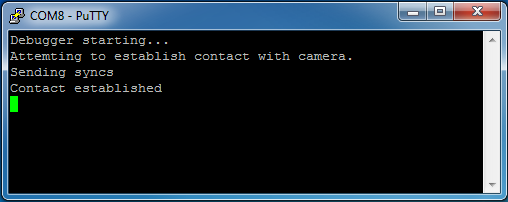
\includegraphics[width=1.0\textwidth]{testing_screenshots/camera_basic_connection_test.png}
        \captionof{figure}{Testing our implementation of the basic connection to the camera module.}
        \label{fig:test_basic_connection}
\end{figure}

Figure \ref{fig:test_basic_connection} shows the result of a test for basic connection to the camera module. In figure \ref{fig:test_basic_connection} the line ``Contact established'' means the Arduino has detected these correct responses. With this successful connection, milestone \ref{sec:ms_basic_cam_comm} is validated, meaning the implementation was free to move on.

\subsection{Test: Image from Camera - (mh)}
\label{sec:image_capture_test}

The first attempt at a simple test for this was to use the debug connection to the Arduino camera controller implementing the camera connection code to relay image data to a PC, unfortunately as described in section \ref{sec:misc_cam_probs} initial implementations of this were not successful, since the debug connection was not completely error free, causing the image to be malformed and unreadable.

However, at this point in the implementation the basic SD card communication had already been implemented and tested as described in section ||||| REF ||||||. Because of this, it was decided  that a much more sensible test would be to write the image data directly to the SD card. The test comprises of running the camera connection code on the microcontroller with the camera and SD card attached. Figure \ref{fig:test_camera_image_saving_sd_card} shows the debug information sent from the controller during this test and \ref{fig:Nyan1} shows the image saved to the SD card. The dedug information suggests that the connection and download of image data was successful and the image on the SD card verifies this.

\begin{figure}[H]
        \centering
        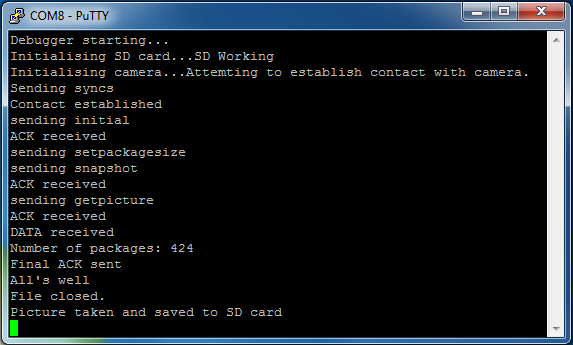
\includegraphics[width=1.00\textwidth]{testing_screenshots/camera_image_saving_sd_card_test.png}
        \captionof{figure}{Debug information sent from camera controller to PC while taking a picture and saving it to an SC card.}
        \label{fig:test_camera_image_saving_sd_card}
\end{figure}

\begin{figure}[H]
        \centering
        \includegraphics[width=1.00\textwidth]{figures/nyanNyan.jpg}
        \captionof{figure}{Test image captured using the Arduino implementation of the camera controller}
        \label{fig:Nyan1}
\end{figure}

The testing during development means that functionality of the controller has been verified already, the test that needs to be performed on this element of the system is to time how long it takes to get an image from the camera and save it to the SD-card and check that this is well within the 3 minutes allowed by the specification. Timing of this process showed that it took around 5 seconds to complete, so well within the 3 minute limit in the specification.

This test verifies milestone \ref{sec:ms_img_from_cam}. The resolution of the image is 640x480.

\subsection{Test: Change Resolution - (mh)}
\label{sec:test_change_resolution}

Since the option to change resolution was a low priority task it was implemented and tested after the basic main system - including image transmission over the autopilot link - was operational.

This test involved sending a Change Camera Resolution command to the payload module over the autopilot link from the ground station, checking the debug line for the correct response and viewing the images downloaded from the camera to verify resolutions.

\begin{figure}[H]
        \centering
        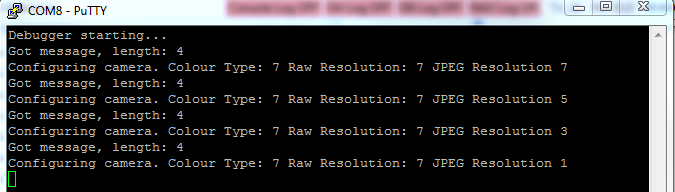
\includegraphics[width=1.00\textwidth]{testing_screenshots/change_res_debug_1.png}
        \captionof{figure}{Test images captured using the integrated implementation of the camera controller}
        \label{fig:test_change_res_debug_1}
\end{figure}

Figure \ref{fig:test_change_res_debug_1} shows the debug information sent from the payload module, the four ``Configuring Camera'' messages in the figure correspond to resolution change messages sent from the ground station. The resolution was changed to the four JPEG resolution values available one after another: 
\begin{itemize}
	\item \textbf{640 x 480}  - Corresponds to ``JPEG Resolution 7''
	\item \textbf{320 x 240} - Corresponds to ``JPEG Resolution 5''
	\item \textbf{160 x 128} - Corresponds to ``JPEG Resolution 3''
	\item \textbf{80 x 64} - Corresponds to ``JPEG Resolution 1''
\end{itemize}

The presence of the debug information recieved from the payload does not validate anything alone, therefore an image was taken at each resolution, shown in figure \ref{fig:change_res_debug}.

This test validates milestones \ref{sec:ms_img_cam_change_res} and \ref{sec:ms_pl_img_gs_cam_res}.

\begin{figure}[H]
  \centering
  \begin{tabular}{c c}
  \subfigure[640 x 480]{\label{fig:whole_fft_lfc}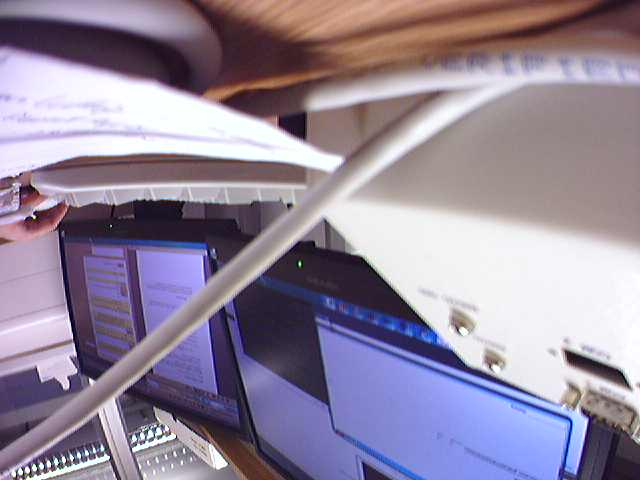
\includegraphics[width=0.5\textwidth]{testing_screenshots/res_pic_640_480.jpg}}&                
  \subfigure[320 x 240]{\label{fig:whole_fft_mfc}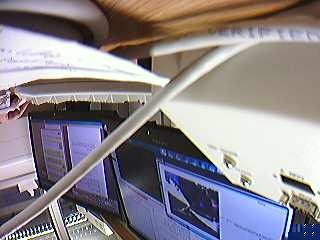
\includegraphics[width=0.25\textwidth]{testing_screenshots/res_pic_320_240.jpg}} \\
  \subfigure[160 x 128]{\label{fig:whole_fft_all}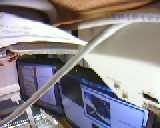
\includegraphics[width=0.125\textwidth]{testing_screenshots/res_pic_160_128.jpg}} &
  \subfigure[80 x 64]{\label{fig:whole_fft_all}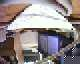
\includegraphics[width=0.0625\textwidth]{testing_screenshots/res_pic_80_64.jpg}}
  \end{tabular}
  \captionof{figure}{Images taken at various resolutions - these were saved by the ground station software after they were downloaded over the autopilot link.}
  \label{fig:change_res_debug}
\end{figure}



%\subsection{Final Camera Testing - (jc)}
%\label{sec:camera_integration_test}

%During the integration process the system was regularly tested for functionality and any errors were fixed as the system was developed. A large number of images were taken during this process and during the implementation of additional features.

%\begin{figure}[H]
    %    \centering
       % 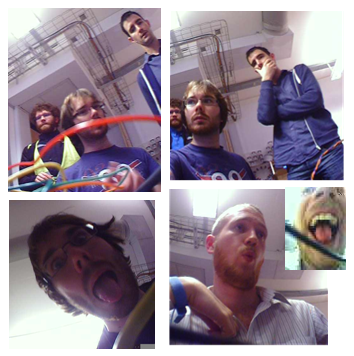
\includegraphics[width=1.00\textwidth]{figures/SampleImages1.png}
       % \captionof{figure}{Test images captured using the integrated implementation of the camera controller}
       % \label{fig:Samples1}
%\end{figure}

%The system can capture images at the 640x480 resolution specified and can also capture images at the other resolutions at which the uCam will take jpeg images. %Currently the option to capture raw images is not implemented.

%The time taken for the system to capture an image at maximum resolution, save it to SD-card and then download and display it on the ground station software was measured at 19.1s |||||||||REF|||||||||. This is still well within the 3 minutes specified and has large amounts of overhead meaning that it should remain well within that limit even if there are+ other payloads implemented on the UAV or if a lot of packets are dropped and have to be resent.



\section{Ground Station Image Viewer(ps26g08)}
\label{sec:ground_station_image_viewer}
The GUI needs a long winded testing. This is because the buttons have to be click and test one by one separately. Because of this, some function of the UAV that does not need a button to test will have its own console application to test it in order to save time. The programmer has to detect most bugs in the real operationThis part is very important because for any program if it caught an error, the program will end unexpectedly.
\subsection{Using Console Application: Testing Connection to UAV, Send Token to Stream Port}
\label{sec:testing_connection_send_to_stream}
The UAV connector use .NET class called System.Net.Sockets. The method that will be using from this class is Sockets.Connect(), Sockets.Send(), Sockets.Receive(). To test the function of this class the programmer develop a separate console application in order to debug only the specific part of the program. Sockets.Connect can be tested by using the Console to display the error code of the running application. The problem could be wrong host name and port number. Therefore, the user are not allowed to change these values. The other problem found in the program is that the programmer forgot to connect the UAV, tell the GCS to enable the enable the network server, and tell the GCS to stream data. Appendix\ref{appen:connectorTest} shows a Connector class that use for testing the Socket connect, read and write method.
Figure \ref{connect to Stream Port} shows a console application testing of the connect function. 
The method is to send a zero token to the data stream and in the GCS program it will display text,\texttt{''\* New datastream client connected from 127.0.0.1:49586''} which it is highlighted in green. 
This text shows that the program works properly and we have accessed to the datastream port of the UAV.
However, the command that send the datastream has not tested in this part. 
This will test the Milestone \ref{sec:ms_basic_dummy_server_comms}.
\begin{figure}[H]
\begin{center}
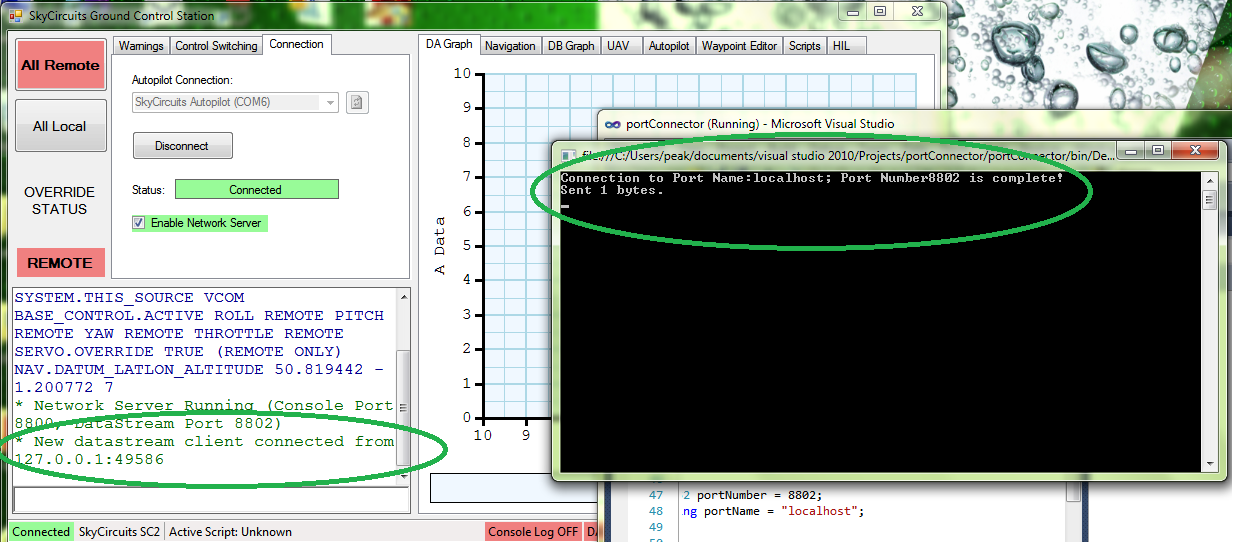
\includegraphics[width=1.00\textwidth]{testing_screenshots/test_sending.png} 
\end{center}
\caption{A screen shot showing the connection with the UAV was successful\label{connect to Stream Port}}
\end{figure}

\subsection{Using Console Application: Testing Connection to UAV, Receive Data from Stream Port}
\label{sec:testing_receive_stream}
Figure\ref{test screenshot} shows a data stream back our testing console application.
Firstly, in the GCS program, we write ''da 30 ht''. 
This code will make the height data stream to the ground station, this data will display on the graph and in the console application, and we can see the number clearly changed when the height has changed.
This is testing that the data stream is working correctly and we have a correct way of getting the data.
Therefore, the Milestone \ref{sec:ms_gs_basestation_comms} is validated.
\begin{figure}[H]
\begin{center}
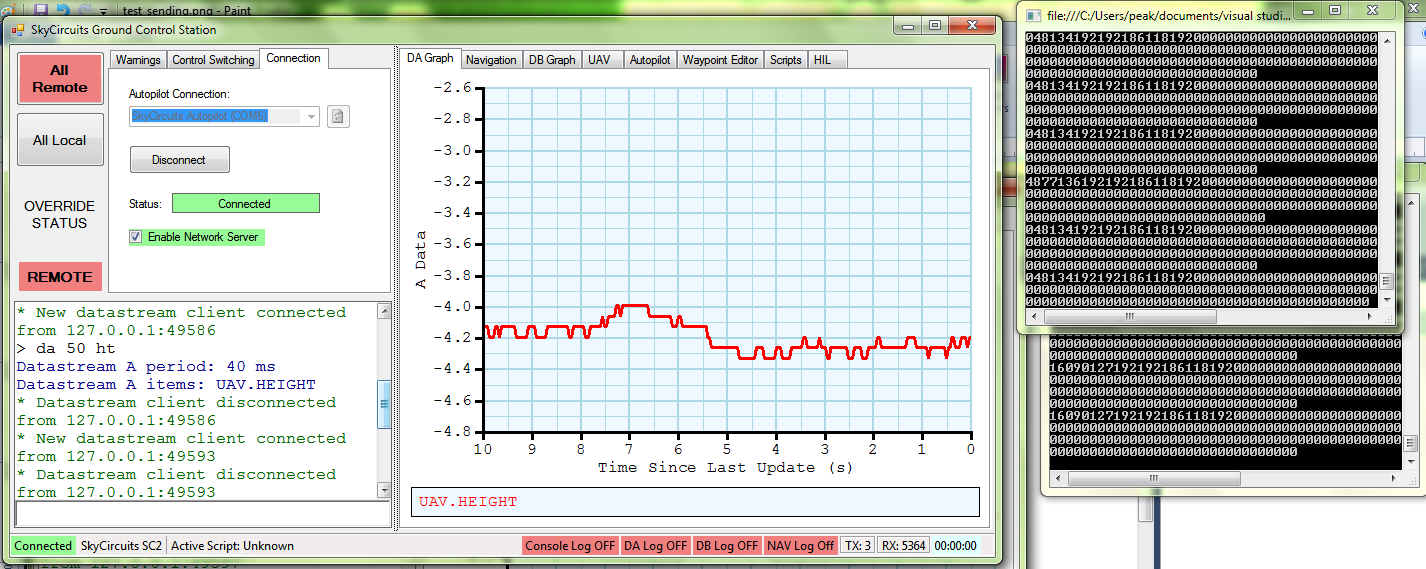
\includegraphics[width=1.00\textwidth]{testing_screenshots/test_data.png} 
\end{center}
\caption{A screen shot shows that the data stream successfully\label{test screenshot}}
\end{figure}

\subsection{Using Console Application: Testing Send Command to Console Port}
\label{sec:send_console}
Figure\ref{test text} show a communication with the console port.
The ground station program allow the programmer to use the console port to send a string command to it. 
This string command can be test that it is correct by the ground station program will produce a line with ''@'' sign on the front of the command sent from the outside of the program.
If the data is correct, the ground station program will detect it and send the data to UAV. 
In the console program, when the user type anything in the console line, it will send byte data to the GCS program.
If the text is a command, the program will process the command and send a byte value as set in the command to the UAV.
The first test is try type 'hi' into the console line.
The GCS will then see the word 'hi' but there is no command available for it.
Therefore, in the GCS console line, it display 'unknown class HELLO'.
Because we send the word via the console line, there is a \@ sign in front of the 'hello' word in GCS program.
The next line we type in is ''da 50 b''.
GCS program know this command therefore it changes the display in the graph to give information about banking of the UAV.
This test validates Milestone\ref{sec:ms_basic_dummy_server_comms}.
\begin{figure}[H]
\begin{center}
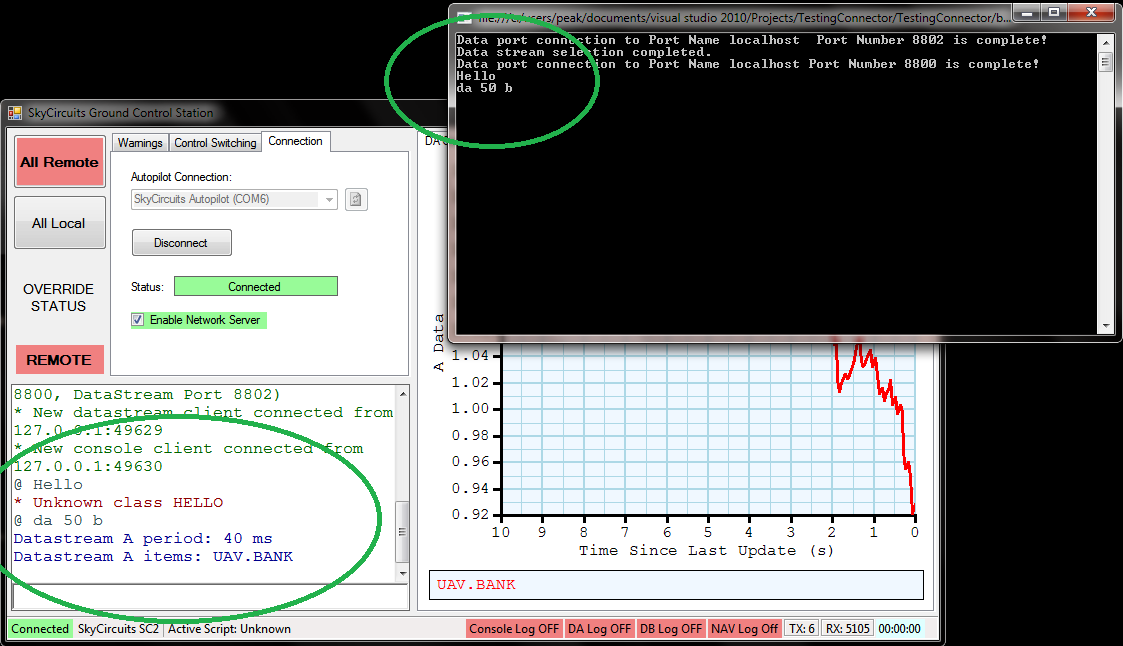
\includegraphics[width=1.00\textwidth]{testing_screenshots/test_sending_test_text_useful.png} 
\end{center}
\caption{A screen shot showing the text sending change the GCS (Ground Control Station) graph value\label{test text}}
\end{figure}

\subsection{Using Window Application: Testing Get Image Button}
\label{sec:test_get_image_button}
The connection between the aircraft and the ground station is using TCP port, it allows the data to send from the aircraft in any form of data. 
In order to test this relationship, a camera will take a picture that the developer know what the picture look like. 
If the picture display an image the same as we expected, the image data is correct.
Figure\ref{camera testing1} shows completed, combined classes together and receive image data.
This testing combined all the existing method together in the Window application.
At this point the connector class will be in the main window application.
When the user click on 'Get Picture' button on the window application, the program will communicate bidirectional, send and receiving which already stated in section\ref{get image algorithm}. 
From the figure, it clearly see that the image is downloading and the image has displayed correctly. This test validates Milestone \ref{sec:ms_gs_recieve_image}. 
\begin{figure}[H]
\begin{center}
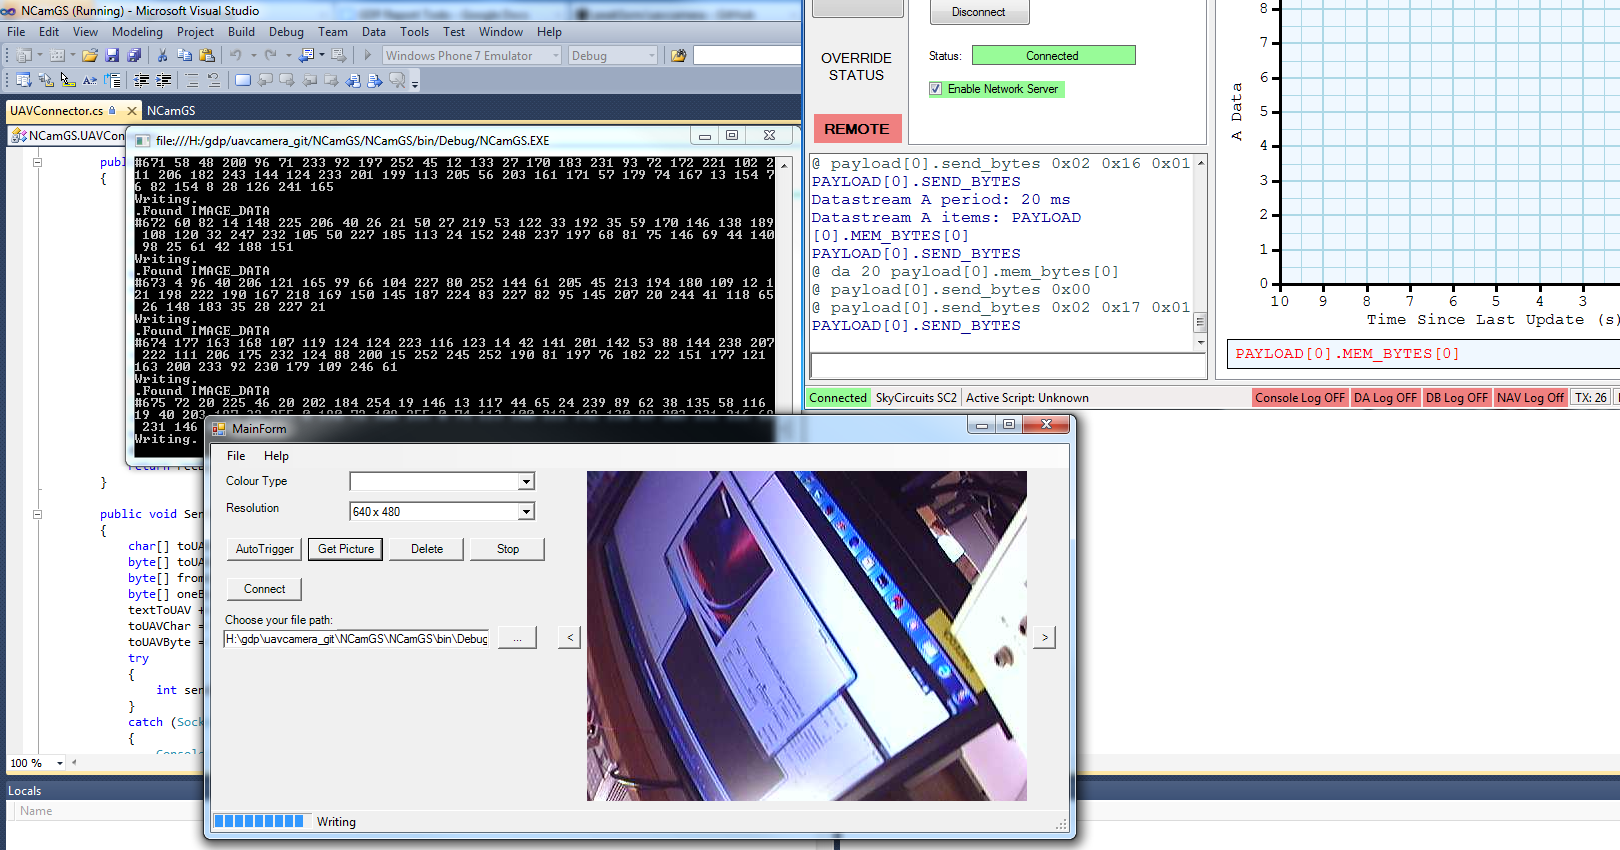
\includegraphics[width=1.00\textwidth]{testing_screenshots/cam_test_11.png} 
\end{center}
\caption{A screen shot showing the picture has been taken correctly\label {camera testing1}}
\end{figure}

\subsection{Using Window Application: Testing Resolution Option}
\label{test_res_op}
When the resolution option changes, the Image viewer program will change the command byte that send to the Console Port of the UAV. 
This can be test by changing the combo box in the image viewer program and click on the Get Picture button.
If it is working correctly, the ground station will see the correct resolution chosen of the picture taken.
Figure \ref{resolution testing} shows a working resolution changing module. 
The putty shows the resolution command that sent back from the payload.
Therefore, it has proved that the resolution option is working.
This test complete the Milestone \ref{sec:ms_pl_img_gs_cam_res}.
\begin{figure}[H]
\begin{center}
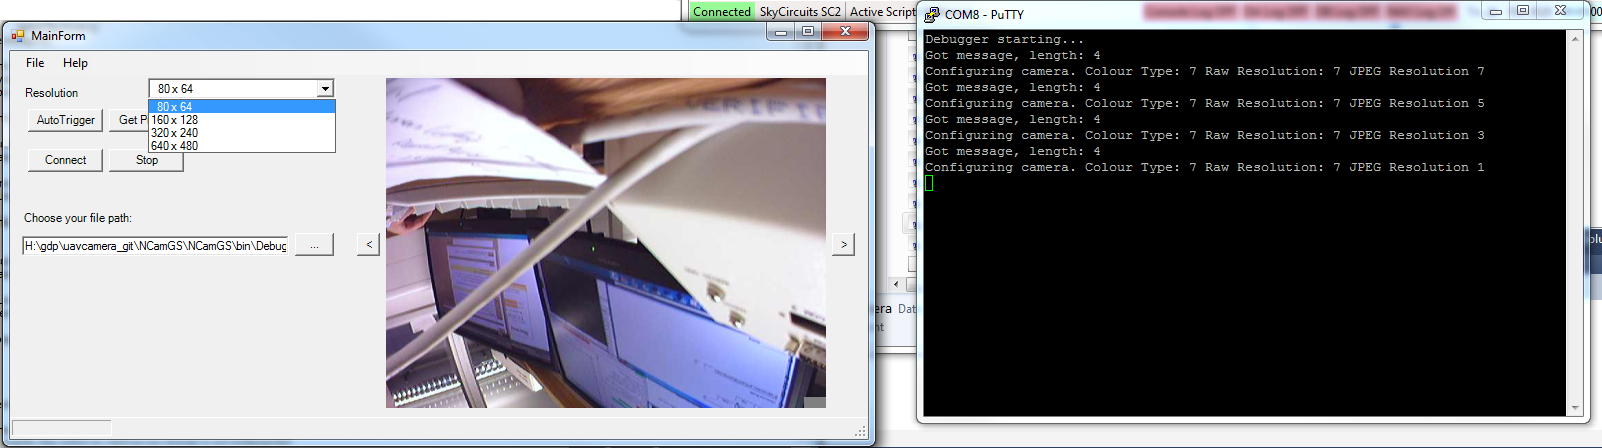
\includegraphics[width=1.00\textwidth]{testing_screenshots/change_res_ncam_1.png} 
\end{center}
\caption{A screen shot showing that the resolution chosen send different signal to the payload\label{resolution testing}}
\end{figure}

\subsection{Functional User Interface}
\label{func_UI}
The tests listed above verifying Milestone \ref{sec:ms_gs_func_interface} is completed. The figure\ref{completeGUI} shows a complete user interface that is functional and ready for the customer to use.
\begin{figure}[H]
\begin{center}
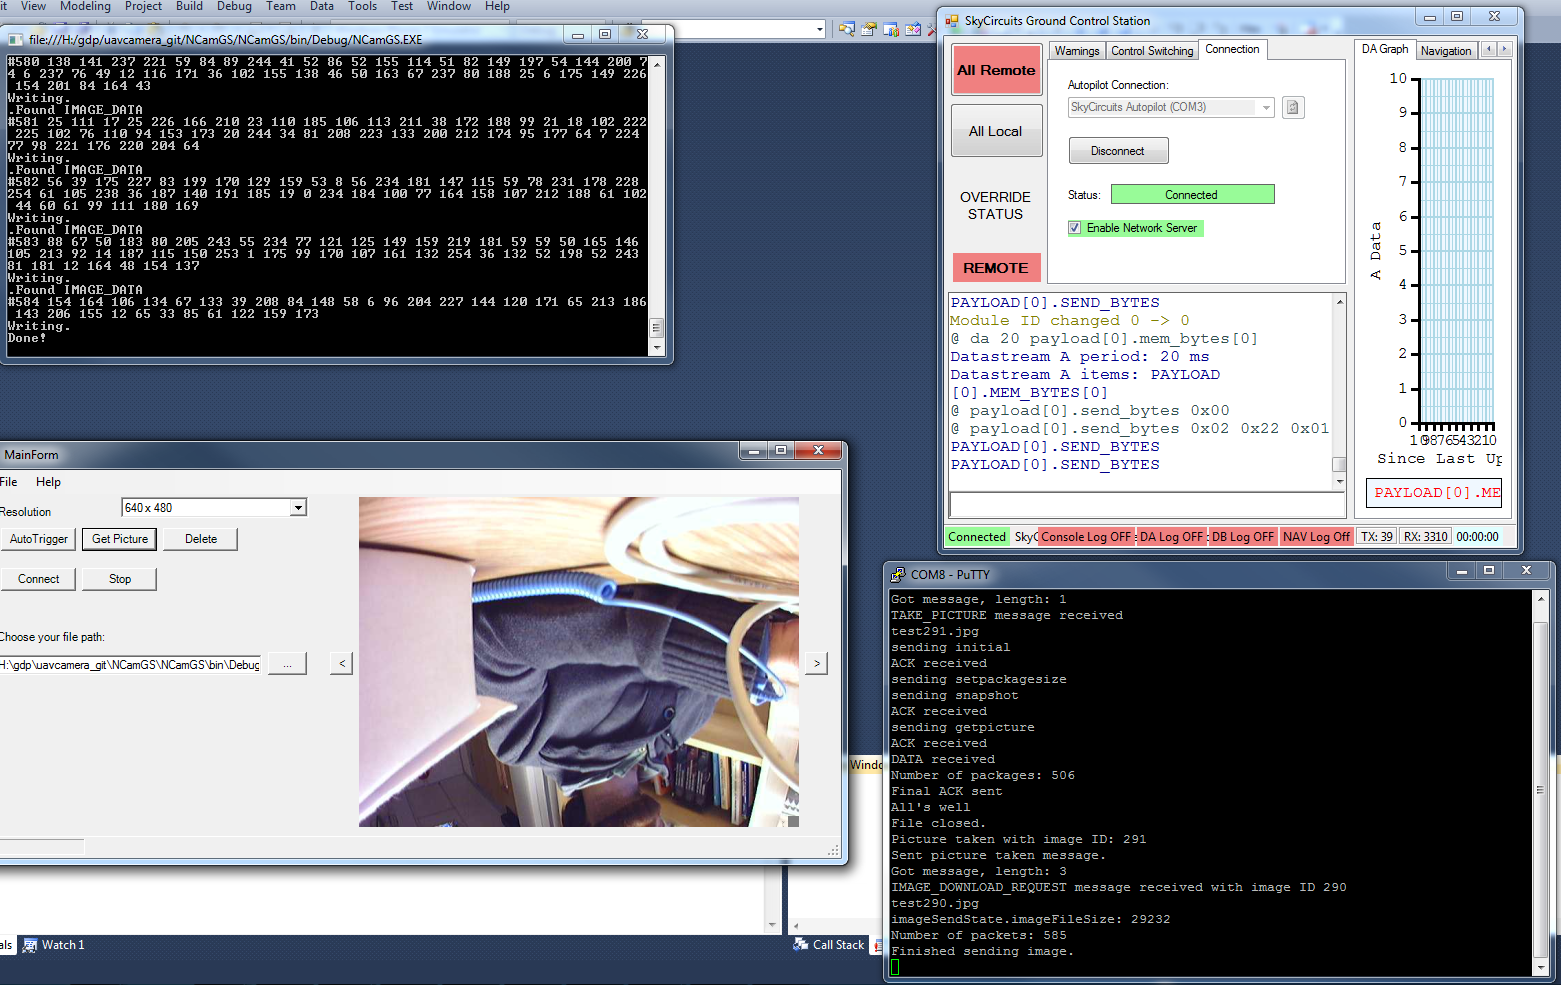
\includegraphics[width=1.00\textwidth]{testing_screenshots/complete_testing_3.png} 
\end{center}
\caption{A screen shot showing a complete UI\label{completeGUI}}
\end{figure}





%% ----------------------------------------------------------------
\section{JPEG Extractor Testing - (ms)}
%% ----------------------------------------------------------------

\subsection{Introduction}

Before the JPEG extractor can be integrated into the
AVR microcontroller, it is necessary to make sure that it is
successful in extracting the header information. This is 
achieved by coding the JPEG extractor as a C executable
file which takes in a JPEG image file and prints out the
information that it will send to the ground station software.

In order to ensure the validity of the information that is 
extracted from the JPEG file, the extractor's output is 
compared against the output of the JPEGsnoop file extractor. 
JPEGsnoop is a free Windows application which takes a 
JPEG image and outputs the information content of all 
of the JPEG file's segments. \cite{hass_impulse_jpeg} 
This software provides a much more 
complete JPEG segment  information extraction and 
includes all the information extracted from the 
created JPEG extractor C executable. This is a sample
output of the JPEGSnoop application applied to the
Leaves2.jpg test image.

\begin{figure}[!hbtp]
\begin{center}
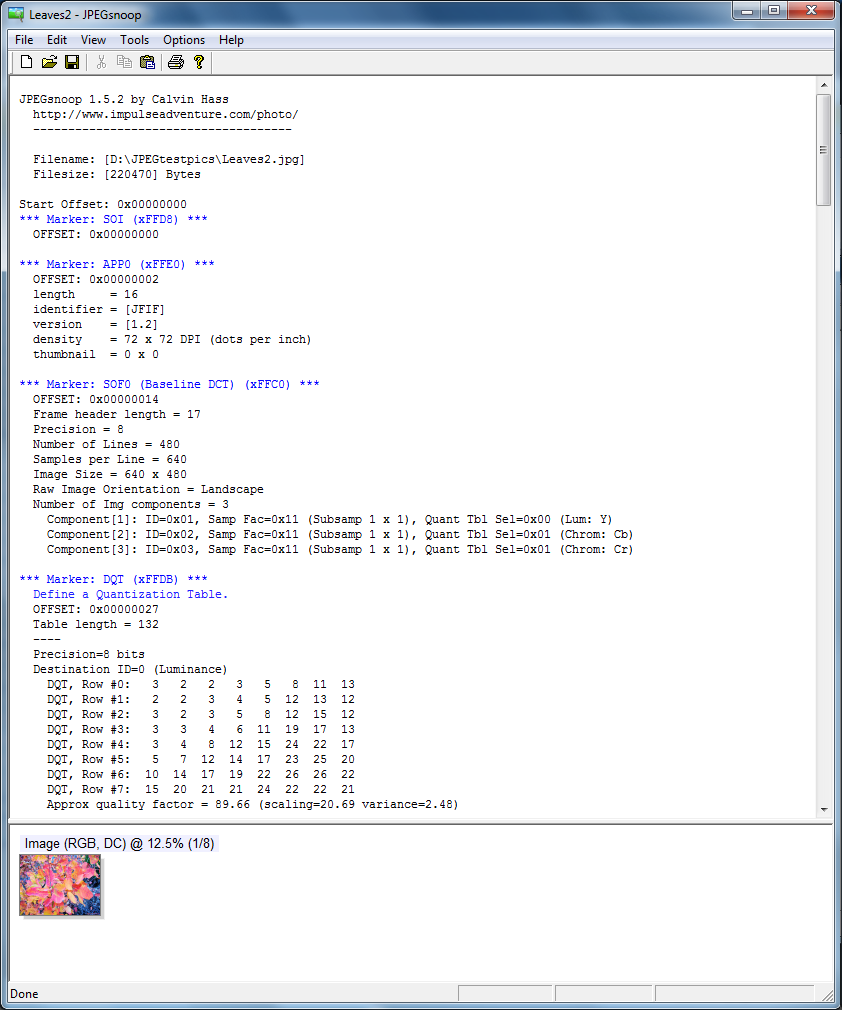
\includegraphics[scale=0.6]{figures/jpegSnoopEx1.png} 
\end{center}
\caption{JPEG segment information obtained from JPEGSnoop.exe}
\end{figure}

\newpage

The images used for the basis of the following tests
were 8 JPEG images of size 640x480 or
less. The pictures are deliberately chosen to be 
complex in order to ensure that the JPEG extractor 
can handle any image given to it by the camera.
The comparison figures below show some of the 
different images used for testing. During all 8 tests,
the output of the C executable was compared with
the output of JPEGSnoop.exe.

\subsection{Test Results}

This section will detail how the C executable's output 
was compared against the output of JPEGSnoop 
for each important JPEG segment. The C 
executable was compiled and run using
the Eclipse development platform and the output
was printed out on the Eclipse console display.

The following segments were tested:

\subsubsection{Test: SOF0}

The SOF0 information is displayed almost
identically between both outputs.
The C executable extractor does not derive the image size nor the
image orientation, because that information will
not be needed for a progressive display of the image.

\newpage

\begin{figure}[!hbtp]
\begin{center}
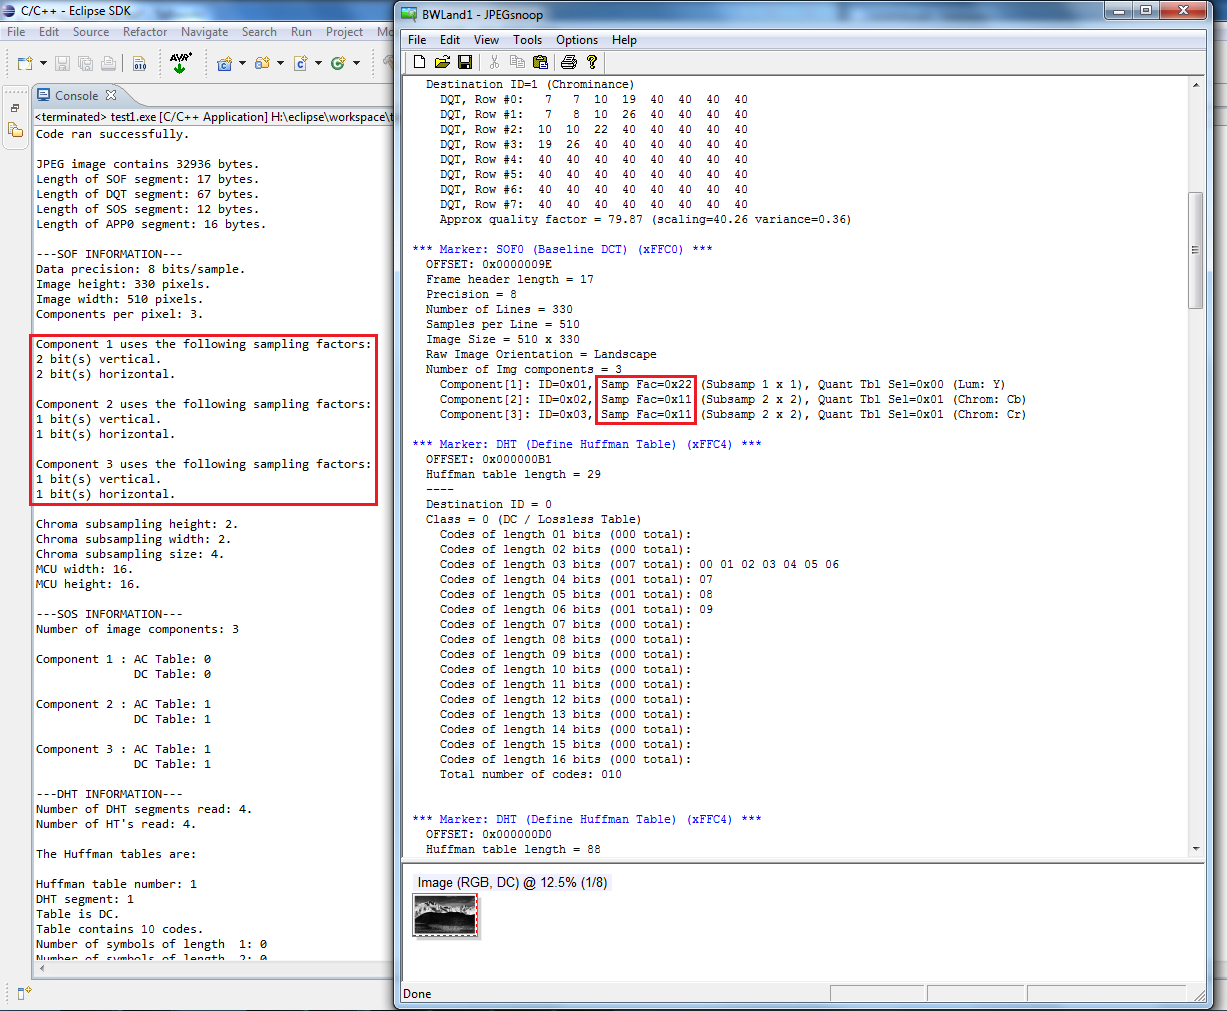
\includegraphics[scale=0.5]{figures/jpegSOFtest.png} 
\end{center}
\caption{SOF0 segment information obtained from JPEGSnoop.exe}
\end{figure}

Note that the sampling factors on each display have
been highlighted with red squares. This is to avoid 
confusion between the sampling factor and the 
subsampling factor.

\subsubsection{Test: DHT}

The extractor keeps track of the DHT segment where the Huffman
table was extracted to better understand the layout of the JPEG
file's DHT segments. The JPEGSnoop extractor simply places the
information in a more compact format compared to the display 
method used by the executable, which has no bearing on the actual
information stored.

\newpage

\begin{figure}[!hbtp]
\label{LeavesImage}
\begin{center}
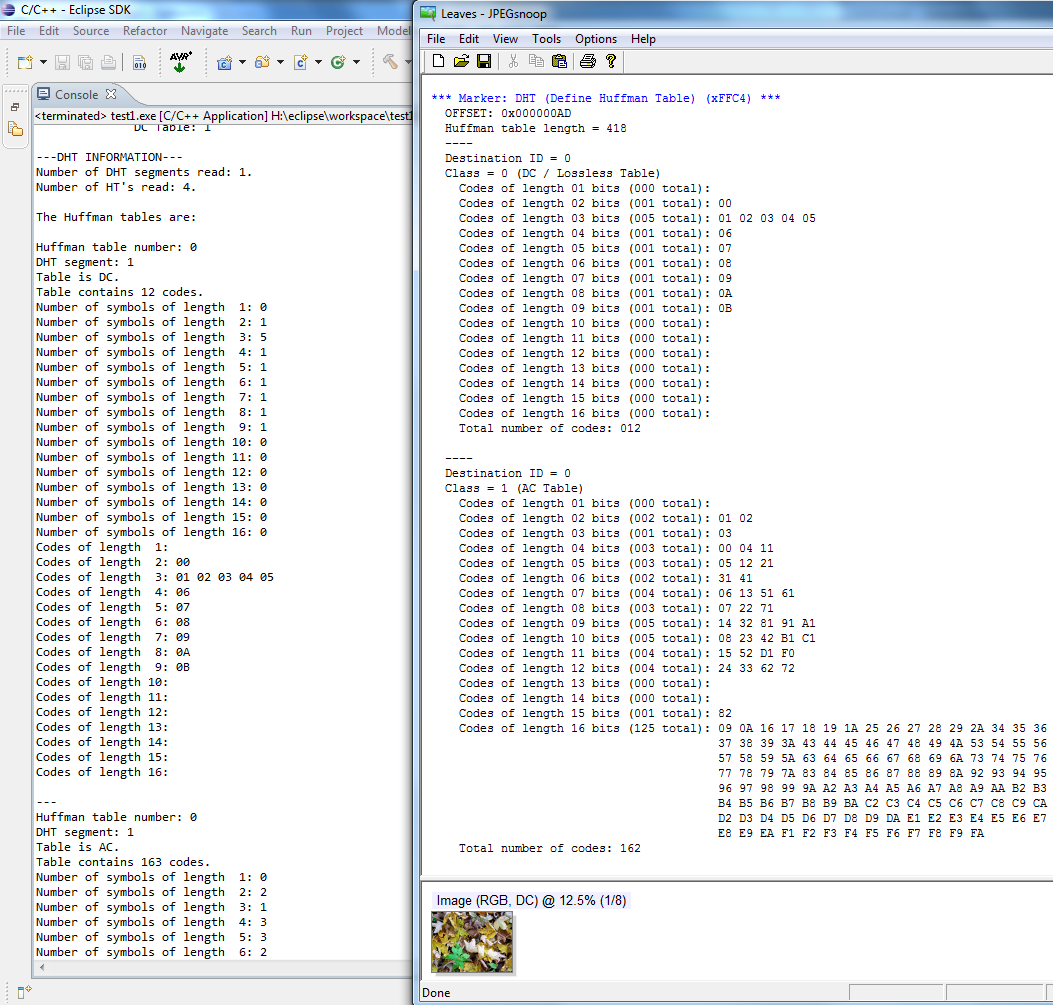
\includegraphics[scale=0.5]{figures/jpegDHTtest1.png} 
\end{center}
\caption{DHT segment information obtained from JPEGSnoop.exe}
\end{figure}

\subsubsection{Test: SOS}

The SOS segment information is read in correctly. The red squares indicate
the DHT tables which are the same in both outputs.

\newpage

\begin{figure}[!hbtp]
\begin{center}
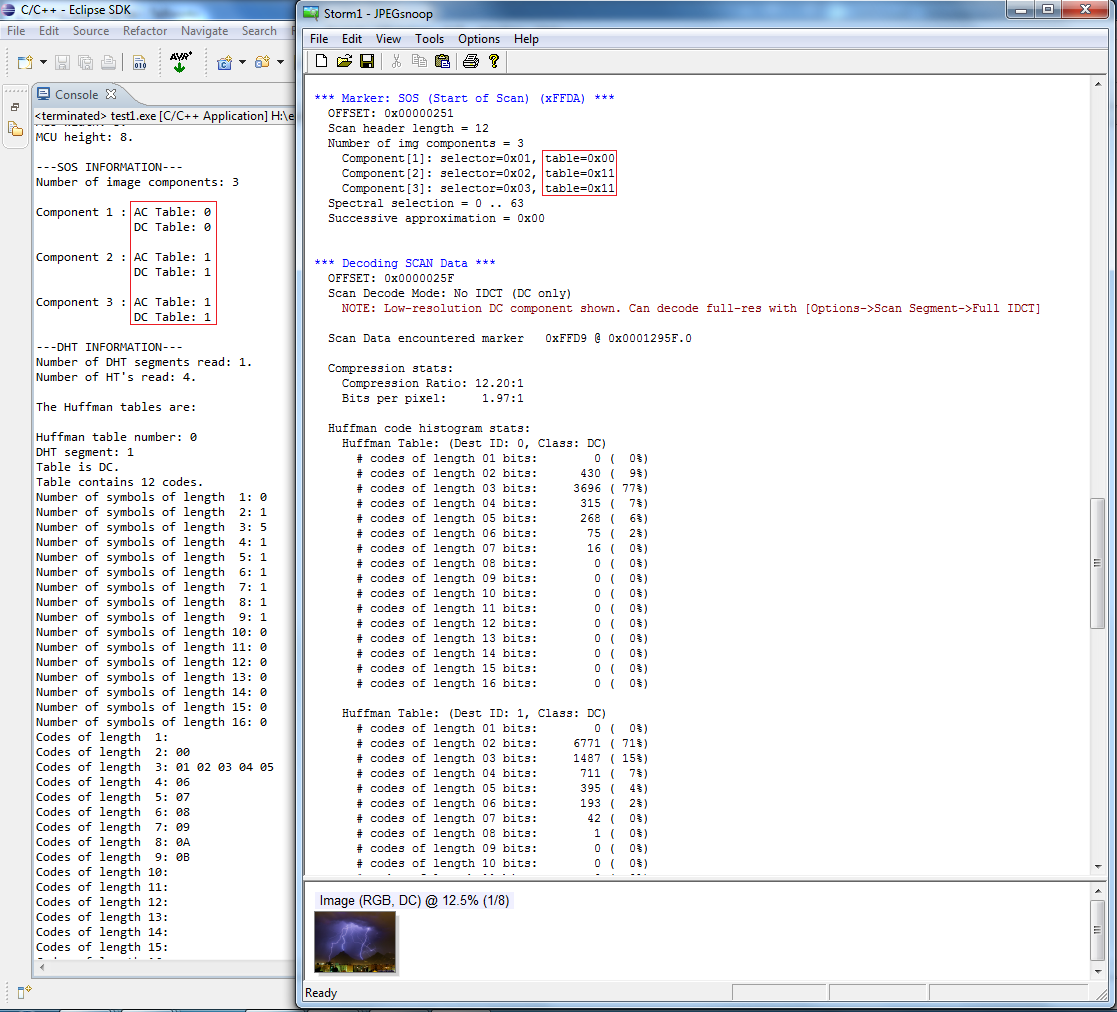
\includegraphics[scale=0.5]{figures/jpegSOStest.png} 
\end{center}
\caption{SOS segment information obtained from JPEGSnoop.exe}
\end{figure}